\begin{frame}
\frametitle{Covert Channel} 
\MakeUppercase{è} un attacco che permette (in 
ambienti ritenuti sicuri) la capacità di comunicare 
o trasferire dati in maniera non autorizzata e non 
voluta. Solitamente sfruttano vulnerabilità o 
comportamenti non previsti nei sistemi per operare 
al di fuori dei soliti meccanismi di comunicazione. 
%Ciò gli permette di non generare segnali di un uso 
%improprio del sistema il che li rende difficili da 
%rilevare. 
\begingroup
\scriptsize
\begin{longtable}{|p{0.25\textwidth}|p{0.7\textwidth}|} 
    \hline
    \textbf{Caratteristica} & \textbf{Descrizione} \\ \hline
    \textbf{Furtività} & Evitare di attirare le 
    attenzioni sia degli amministratori che degli 
    strumenti di sicurezza. \\ \hline 
    \textbf{Capacità di trasmissione} & La quantità 
    di dati che il canale riesce a trasmette. Una 
    quantità elevata può portare ad una rilevazione 
    del canale. \\ \hline
    \textbf{Uso delle risorse} & Un uso delle risorse 
    improprio (o sproporzionato) potrebbe andare in 
    conflitto con le risorse legittime presenti nel 
    sistema. \\ \hline
    \textbf{Rumore} & L'uso dei servizi e/o delle 
    risorse nel sistema potrebbe alterare il loro 
    funzionamento. \\ \hline
    \textbf{Indistinguibilità} & La trasmissione dei 
    dati mantiene inalterato il funzionamento delle 
    risorse utilizzate. Ovvero il canale è 
    indistinguibile dalla risorsa usata. \\  \hline 
\caption{Caratterisitche di un Covert Channel}  
\end{longtable} 
\endgroup
\end{frame} 
%\begin{frame} 
%\frametitle{Furtività DA CANCELLARE} 
%\begin{figure} 
%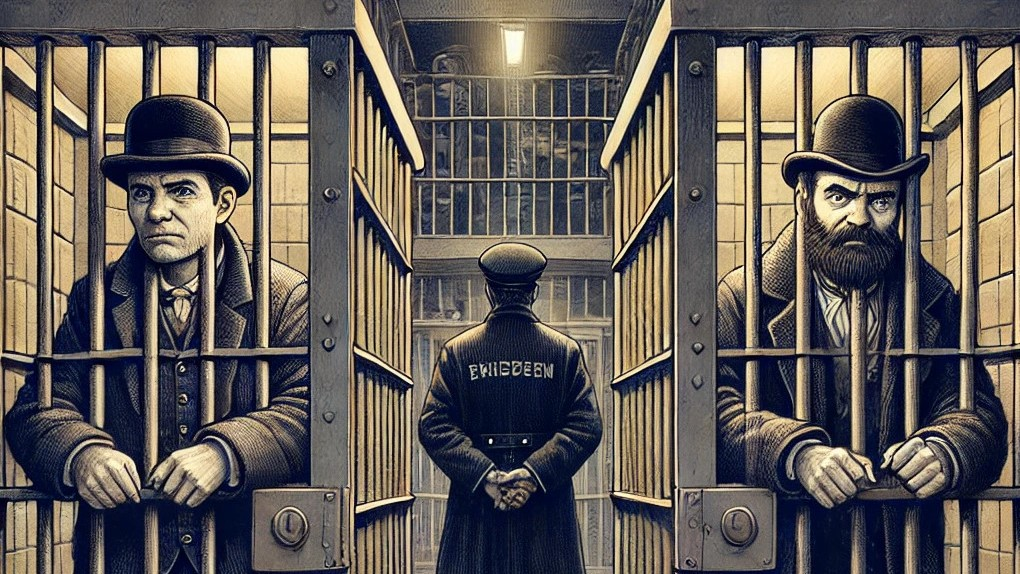
\includegraphics[width=0.8\linewidth]{../Tesi/img/presentazione/thiefs_and_warden_crop.jpg}
%\end{figure}
%%\centering 
%%\justifying
%\MakeUppercase{è} la capacità di evitare di attirare 
%attenzioni indesiderate sia da parte degli 
%amministratori che degli strumenti di sicurezza. 
%\end{frame} 
%\begin{frame} 
%\frametitle{Capacità di trasmissione DA CANCELLARE} 
%\begin{columns}[T,onlytextwidth]
%\column{0.48\textwidth}
%    \begin{figure}
%    \centering
%    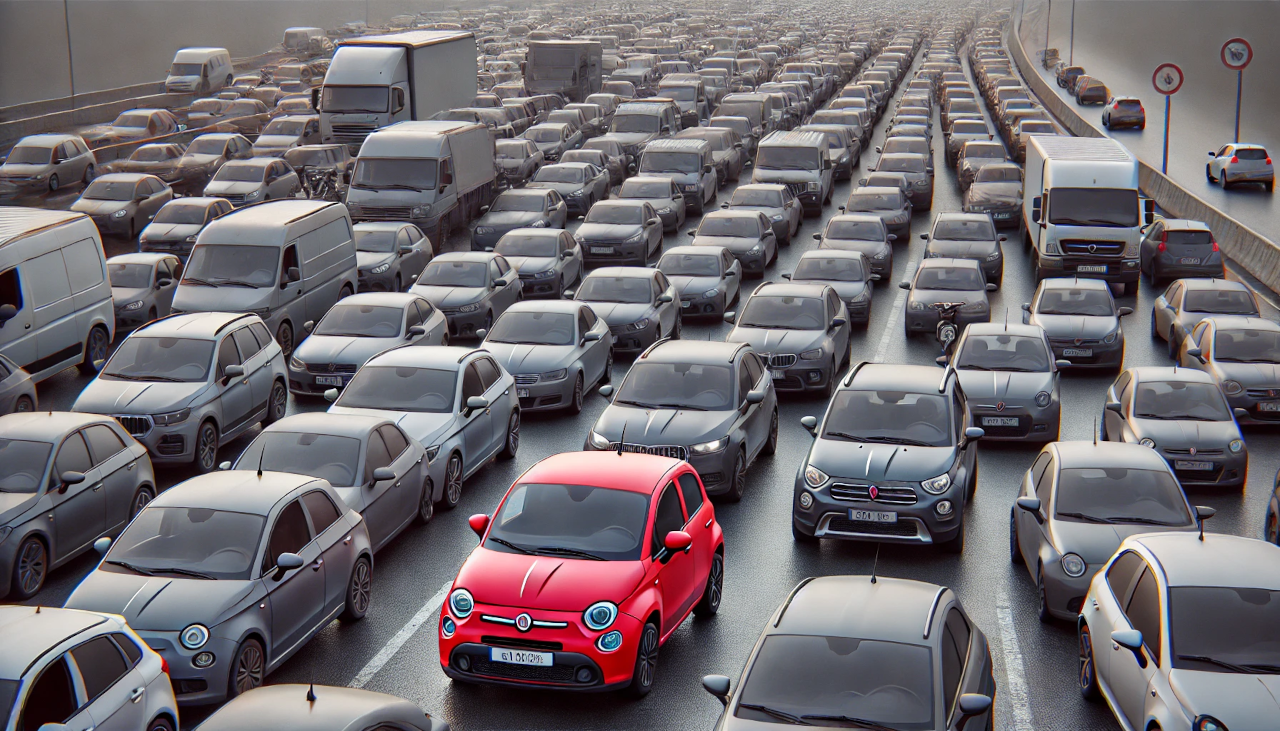
\includegraphics[width=\linewidth]{../Tesi/img/presentazione/covertChanne-pandaRossa.png}
%    \end{figure}
%\column{0.48\textwidth}
 %   \begin{figure}
%    \centering
%    %\includegraphics[height=0.6\textheight]{image1.png}
%    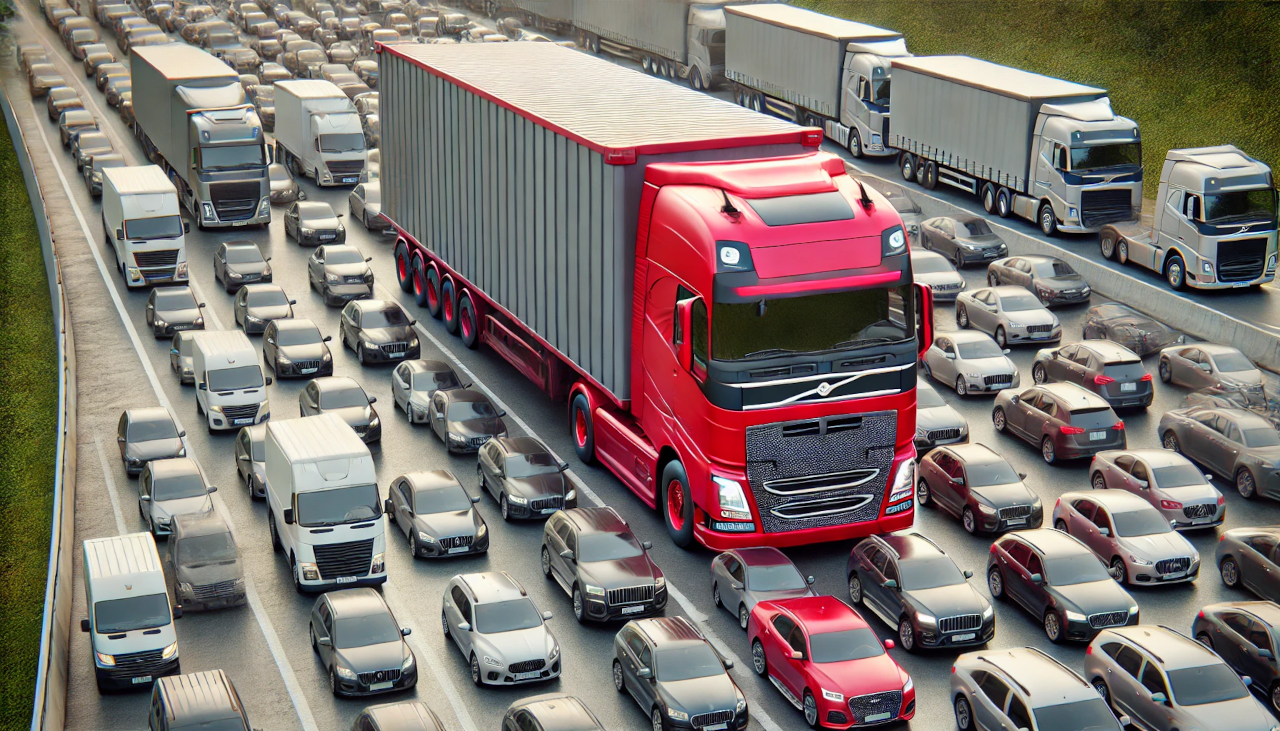
\includegraphics[width=\linewidth]{../Tesi/img/presentazione/covertChannel-camionRosso.png}
%\end{figure}
%\end{columns} 
%\vspace{4ex} 
%\centering 
%%\justifying
%Rappresenta la quantità di dati che il canale riesce 
%a trasmettere. 
%\end{frame}
%\begin{frame} 
%    \frametitle{Uso delle risorse e Rumore} 
%    \begin{columns}[T,onlytextwidth]
%    \column{0.48\textwidth}
%    \begin{figure}
%    \centering
%    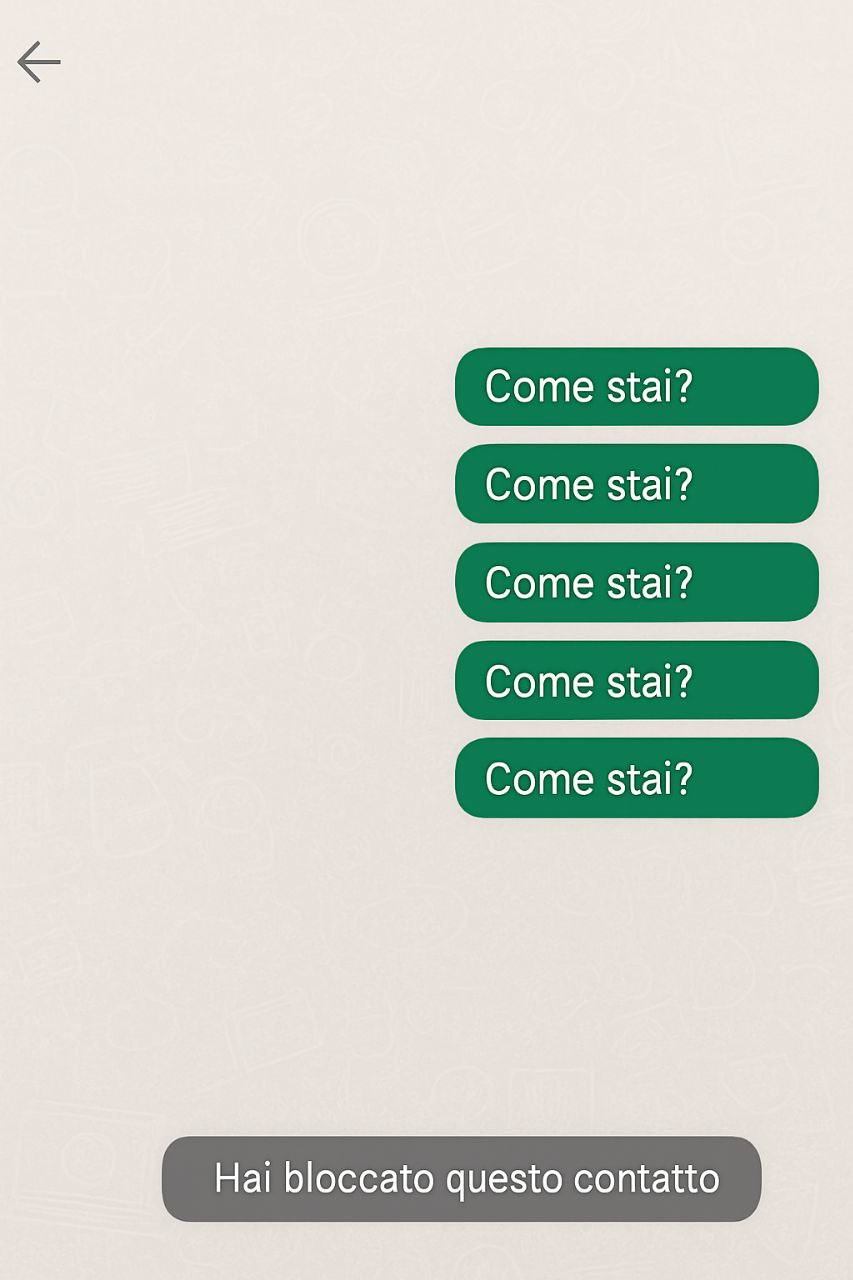
\includegraphics[width=0.7\linewidth]{../Tesi/img/presentazione/5855191149722061057.jpg}
%    \end{figure}
%    \column{0.48\textwidth}
%    \begin{figure}
%    \centering
    %\includegraphics[height=0.6\textheight]{image1.png}
%    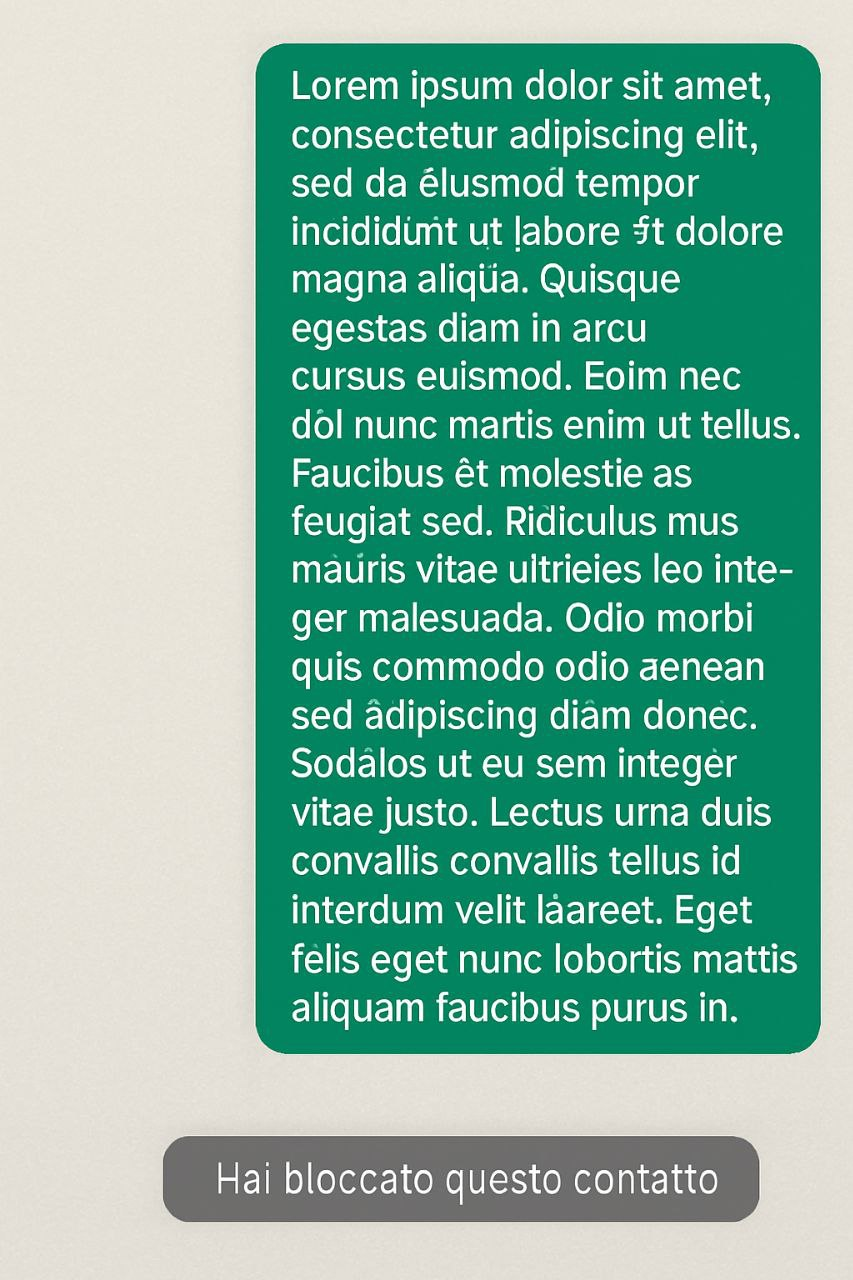
\includegraphics[width=0.7\linewidth]{../Tesi/img/presentazione/5855191149722061058.jpg}
%    \end{figure}
%    \end{columns}
%\end{frame}  
\begin{frame} 
%\frametitle{Indistinguibilità DA CANCELLARE} 
\frametitle{Caratteristiche di un Covert Channel} 
\begin{figure}
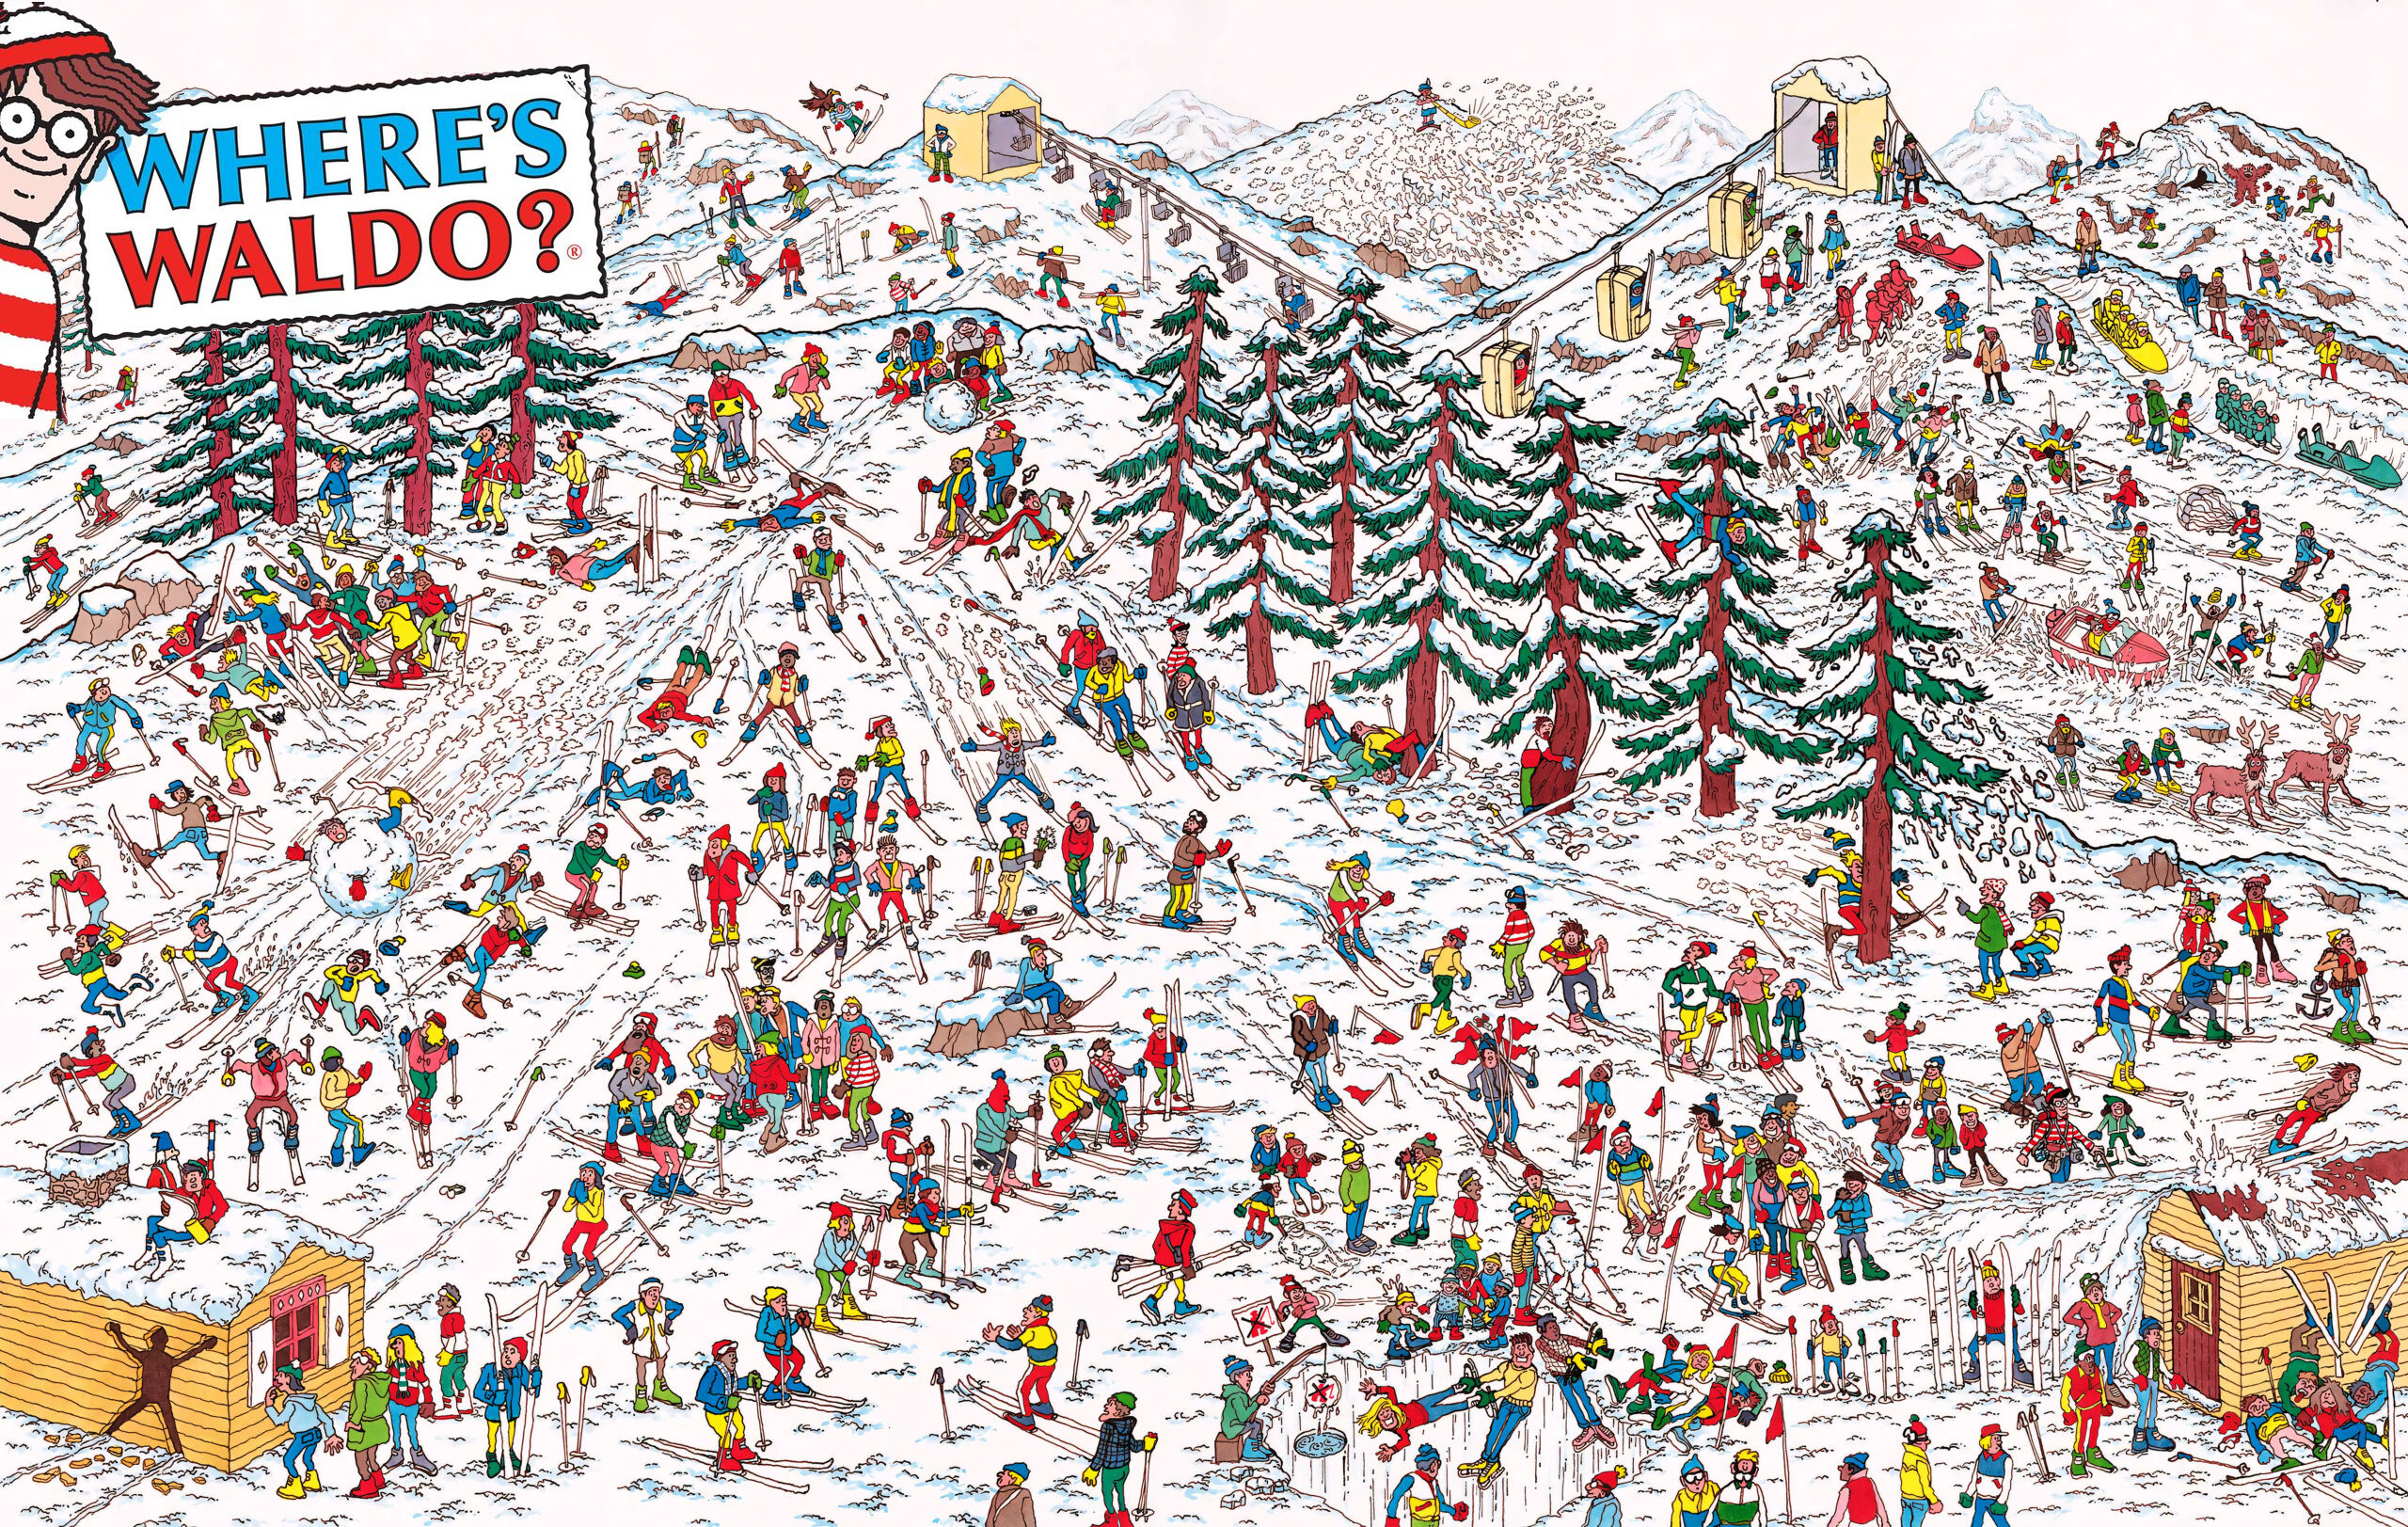
\includegraphics[width=0.85\linewidth]{../Tesi/img/presentazione/wheres-waldo-picture-8.jpg}
\end{figure} 
\begin{center}
%\begin{minipage}{0.8\linewidth}
%\justifying
%Il funzionamento delle risorse utilizzate rimane invariato. 
%\newline
%Ovvero il canale si rende indistinguibile dalla risorsa usata.
%\end{minipage} 
\end{center}
\end{frame}

\begin{frame}
\frametitle{Timing Covert Channel} 
\begin{columns}[T,onlytextwidth]
\column{0.48\textwidth} 
\justifying
I \textbf{Timing Covert Channel} sono metodi di 
comunicazione che permettono ad un osservatore 
(e.g una persona od un processo) di acquisire 
informazioni attraverso il cambiamento del tempo di 
risposta di una risorsa. 
\vspace{2ex} \newline
Qualsiasi metodo che 
utilizzi un orologio (o che misuri il tempo) può 
implementare questa tipologia di canale.
\column{0.48\textwidth} 
%\begin{figure}
\centering 
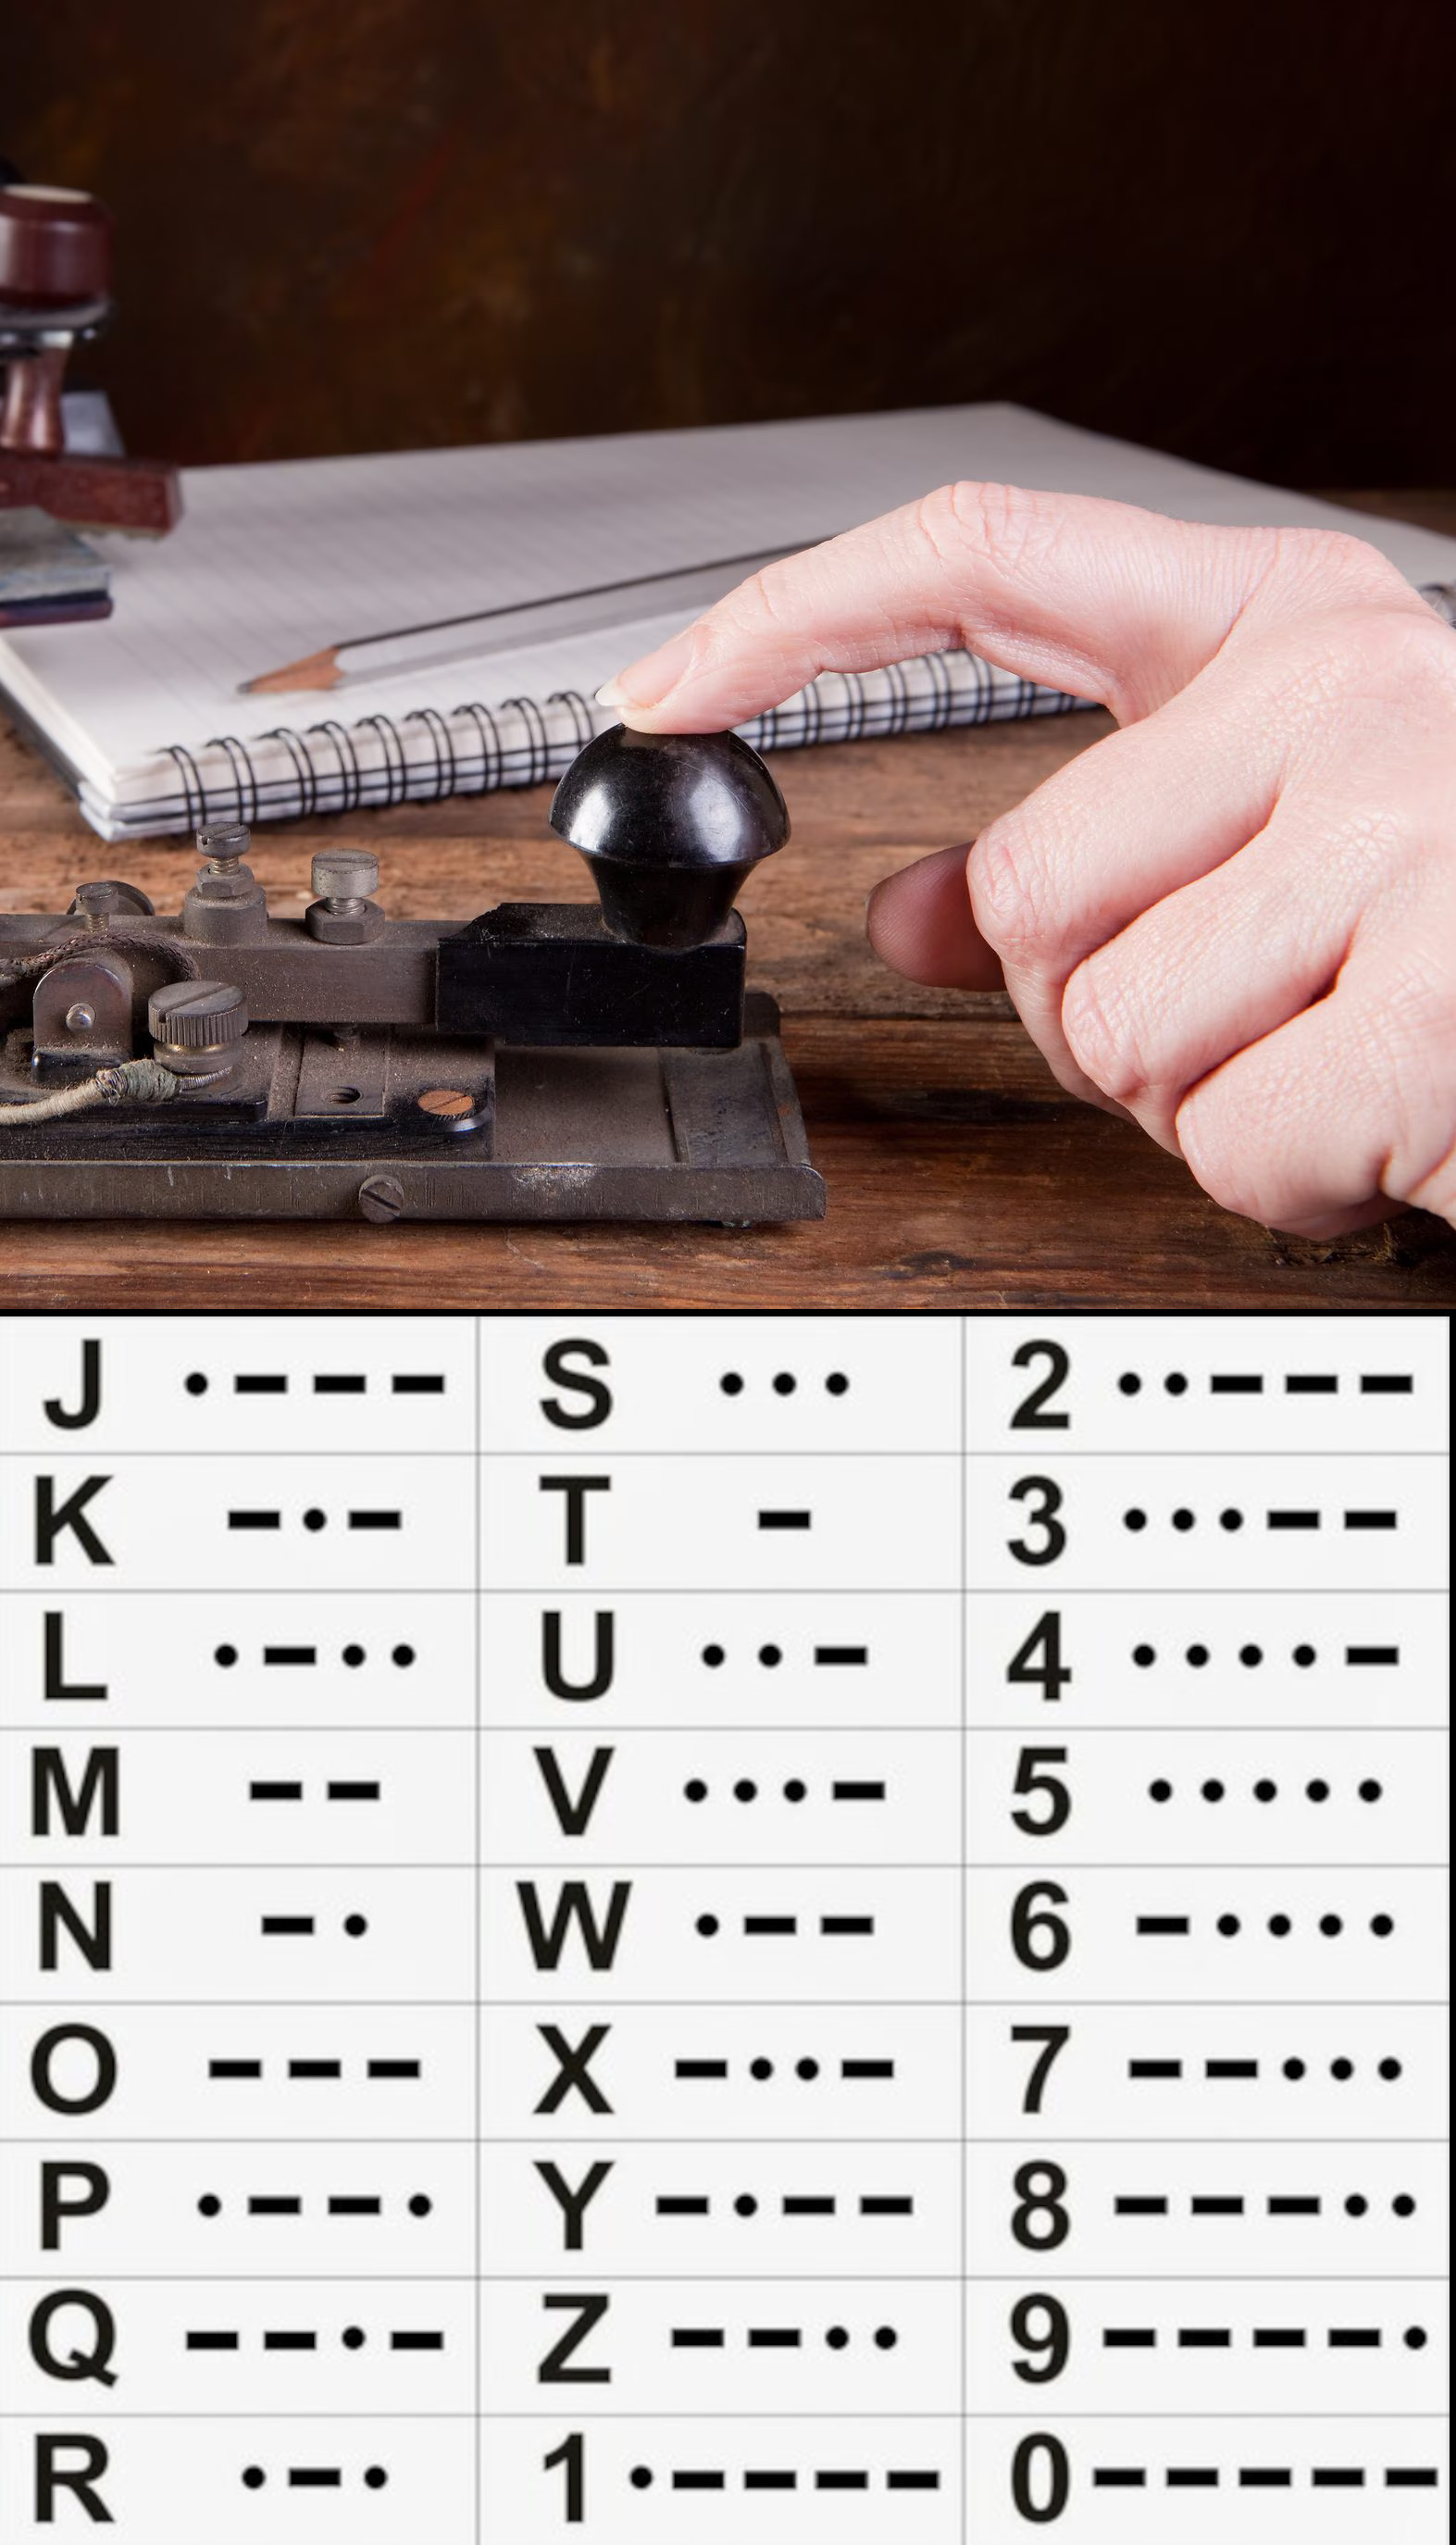
\includegraphics[width=0.8\textwidth]{../Tesi/img/telegrafo2.jpg} 
%\captionof{figure}{Codice Morse} 
%\end{figure}
\end{columns}
\end{frame} 

\begin{frame}[fragile]
\frametitle{Storage Covert Channel} 
\begin{columns}[T,onlytextwidth]
\column{0.48\textwidth}  
\justifying 
Uno \textbf{Storage Covert Channel} scrive dei dati 
su un'area di memoria condivisa accessibile da 
tutte le entità coinvolte nella comunicazione. 
\vspace{2ex} \newline
I veicoli per la sua implementazione saranno tutte 
quelle risorse che consentiranno la scrittura e la 
lettura sulla risorsa condivisa.
\column{0.48\textwidth} 
%\begin{figure}
\centering 
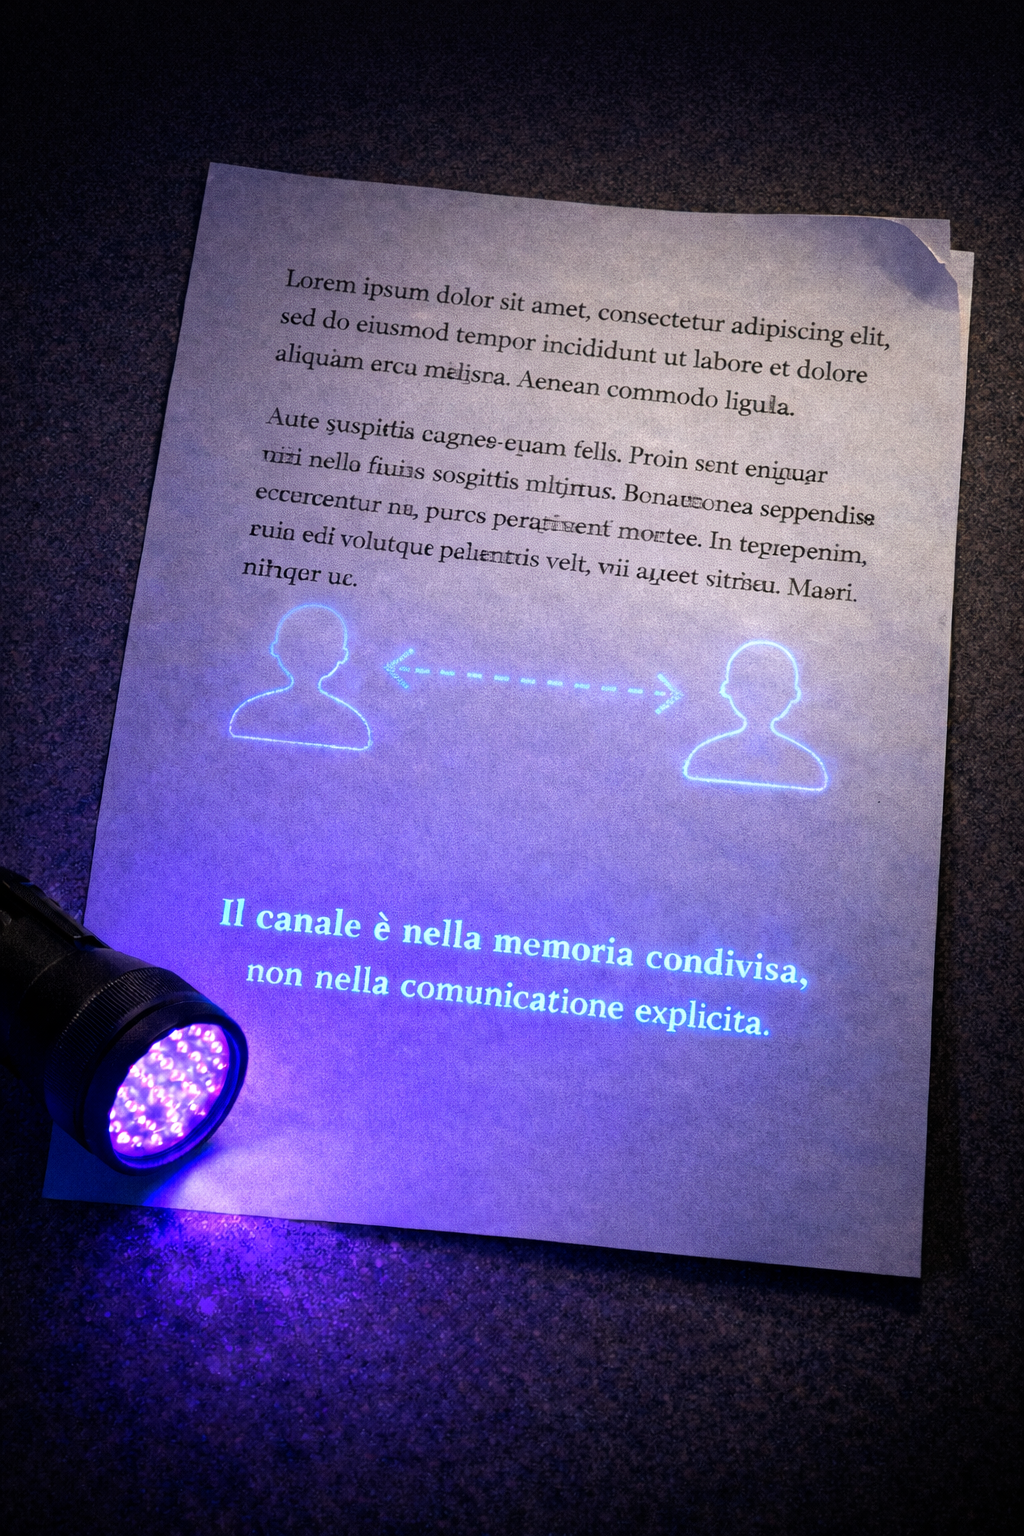
\includegraphics[width=0.65\textwidth]{../Tesi/img/ICMP_storageCC/documento_inchiostrosimpatico.png} 
%\captionof{figure}{Cdocumento con inchiostro simpatico} 
%\end{figure} 
\end{columns}  
\end{frame} 

\begin{frame}
\frametitle{Behavioural Covert Channel} 
\begin{columns}[T,onlytextwidth]
\column{0.48\textwidth} 
\justifying
Nei \textbf{Behavioural Covert Channel} le 
informazioni vengono codificate mediante la 
variazione del comportamento del sitema. 
\vspace{2ex} \newline
I dati verranno quindi ricavati tramite l'osservazione 
del sistema piuttosto che attraverso l'accesso 
(diretto o indiretto) alla memoria.
\column{0.48\textwidth} 
%\begin{figure}
\centering 
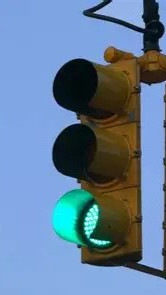
\includegraphics[width=\textwidth]{../Tesi/img/ICMP_behaveCC/semaforo.jpg} 
%\captionof{figure}{Hex dump di un paccheto} 
%\end{figure}
\end{columns}
\end{frame} 

%\begin{frame}
%\frametitle{Tipologie di Covert Channel}  
%\subsubsection{Hybrid Covert Channel} 
%Un Hybrid Covert Channel combina più tecniche per aumentare la capacità di trasmissione dei 
%dati nascosti e rendere più difficile la loro rilevazione. 
%\end{frame}